\documentclass{emulateapj}
%\documentclass[12pt,preprint]{aastex}

\usepackage{graphicx}
\usepackage{float}
\usepackage{amsmath}
\usepackage{hyperref}
\usepackage[caption=false]{subfig}
\usepackage{epsfig,floatflt}



\begin{document}

\title{A spectacular title}

\author{Daniel Heinesen}

\email{daniel.heinesen@sf-nett.no}

\altaffiltext{1}{Institute of Theoretical Astrophysics, University of
  Oslo, P.O.\ Box 1029 Blindern, N-0315 Oslo, Norway}


%\date{Received - / Accepted -}

\begin{abstract}
In this letter we are using the 4 year data from the Cosmic Background Explorer (COBE), and comparing it with the power-law model for the power spectrum. We are looking to find values for the temperature amplitude fluctuation $Q$ and tilt $n$ predicted by inflation theory. We are looking at the $53$ GHz and $90$ GHZ maps of the Cosmic Microwave Background(CMB), removing noise and foreground pollution so only to get signal from the CMB. From this data, and a covariance matrix made from the data and expected models we do a Markov Chain Monte Carlo simulation to get the values of $Q$ and $n$ most in line with the observed data. Through our analysis we obtain $Q = (16.3 \pm 3.81)\mu K$ for $53$ GHz and $Q = (18.9 \pm 6.12)\mu K$ for $90$ GHz, and $n = 0.696 \pm 0.381$ for $53$ GHz and $0.915 \pm 0.623$ for $90$ GHz. This indicates that there were perturbations in the primordial universe, giving rise to temperature fluctuations, and that inflation theories prediction of $n \simeq 1$ is consistent with the observed CMB.
\end{abstract}
\keywords{cosmic microwave background --- cosmology: observations --- methods: statistical, Markov Chain Monte Carlo, Metropolis-Hastings}

\section{Introduction}
\label{sec:introduction}

Since its discovery in 1964 \citep{wilson} the Cosmic Microwave Background (CMB) radiation has been an important field of research in cosmology. The CMB is the red shifted remains of the photons made about 380 000 years after the Big Bang, when the plasma of the primordial universe had cold down enough to be transparent and light could escape. The CMB can now be observed as a $\sim 2.7$ K blanket of microwave radiation covering the whole sky. This radiation was at first shown to behave more or less like a black body. Early Big Bang models expected this radiation to be homogeneous across the whole sky, but in the 60's and 70's a theoretical basis for permutations in the primordial background radiation was found\citep{sunyaev}, which would lead to a small fluctuation in the observable CMB(anisotropy) on the order
\begin{equation}
{\Delta T}/{T} \approx 10 \mu K.
\end{equation} These fluctuations predicted to be both isotropic and Gaussian. This is a clear testable prediction of inflationary theory. 

An other prediction of the inflationary model is that these fluctuations would be nearly the same across all scales $n\simeq1$\citep{zeldovich}. 

The Cosmic Background Explorer (COBE) was mission launched in 1989 by NASA, and collected data to 1993. The satellite was launched with three onboard instruments: the "Far-InfraRed Absolute Spectrophotometer(FIRAS)", the "Diffuse InfraRed Background Experiment(DIRBE)" and the "Differential Microwave Radiometer(DMR)". The latter being of interest in this Letter.

We are going to use the four year $53$ GHz and $90$ GHz maps from the COBE-DMR. We are going to use these maps to estimate the values of the fluctuations of the temperature of the CMB, given by the parameter $Q$; and these fluctuations dependence on scale, given by the parameter $n$.

We are going to use a power-law model for the power spectrum \ref{sec:theory} to estimate a theoretical covariance matrix for data for the parameter $Q$ and $n$\eqref{eq:C(Q,n)}. We are then going apply Bayesian analysis to this covariance matrix calculate the posterior probability that this model is correct given the data obtained from COBE-DMR. We are then going to use a Markov Chain Monte Carlo simulation to optimize these parameters to find the best possible parameters $Q$ and $n$. 

We are only going to look at fluctuations with modes with an effective wavelength\ref{sec:theory} of $\ell \leq 47$, since for these mode the fluctuations are a direct product of the inflation, and thus gives clear evidence for the model \citep{HKforelesning}. Since COBE-DMR only measures the difference between points in the sky, there is a difficulty in measuring monopoles. It also faces problems with dipoles, since motions trough space causes red-shifts in monopoles, manifesting as dipoles; thus making observations of dipoles more likely to originate from this effect than from actual dipoles. Thus we are only looking at multipoles of order $2 \leq \ell \leq 47$.

Should we be able to values for $Q$ and $n$ is line with the prediction of the inflationary model, this would be an important confirmation of the model, and would go a long way of cementing its role as the leading model of the expansion of the universe.


\section{Background Theory}
\label{sec:theory}

The fluctuations in the CMB can be described with the multipole expansion

\begin{equation}
\Delta T(\hat{n}) = \sum_{\ell = 0}^{\ell_{max}}\sum_{m = -\ell}^\ell a_{\ell m}Y_{\ell m},
\end{equation}
where $a_{\ell m}$ is the amplitude of the different modes of the spherical harmonics $Y_{\ell m}$. $\ell$ is the effective wavelength $\ell = 180/\lambda$, and $m$ is the phase. From this we can find the power spectrum defined though the variance of $a_{\ell m}$

\begin{equation}
\langle a_{\ell m}a_{\ell'm'}\rangle = \delta_{\ell \ell '}\delta_{m m'}C_\ell.
\end{equation}

Where $C_\ell = |a_\ell|^2/(2\ell + 1)$ is the power spectrum. This is where our investigation starts. Inflationary theory predicts that in the areas mapped out by COBE-DMR, this power spectrum should follow power law of the form

\begin{equation}
P(k) \propto k^n,
\end{equation}

where $n$ should be a bit smaller than $1$. This makes it possible to parametrize the power spectrum with the parameters $Q$ and $n$, where $Q$ is the amplitudes of the fluctuations, and $n$ is the spectral index and describes the fluctuations dependence on the scale.


%Discuss background, physical importance and possibly some history of
%the problem that is being studied in this paper.


\section{Method}
The method described here is a taken from \cite{oppgave}. For a more detailed description we refer you to that paper.
\label{sec:method}

\subsection{Data Model}
The data from the COBE-DRM is on the form
\begin{equation}
d(\hat{n}) = s(\hat{n}) + f(\hat{n}) + n(\hat{n}),
\end{equation}
where $f$ is the foreground radiation, $n$ is the instrumental noise and $s$ is the actual signal from the CMB.

As mentioned in the introduction, the fluctuations can be taken as Gaussian, so we can expect that the distribution of the real signal in the data goes like
\begin{equation}
p(\mathbf{d}) = \frac{1}{\sqrt{|\mathbf{C}|}}e^{-\frac{1}{2}\mathbf{d}^T \mathbf{C}^{-1}\mathbf{d}}.
\label{eq:prob}
 \end{equation} 

Here $\mathbf{d}$ is the observed data, and $\mathbf{C}$ the covariance matrix for the pixels in the data. The covariance matrix is a quantity that describes how much the signal for each pixel is correlated to the others. The covariance matrix contains all the relevant information of the data we need. We expect that $s$,$f$ and $n$ is non-correlated, and we can therefore write the covariance matrix for the data $d$ as 
\begin{equation}
\mathbf{C} = \langle \mathbf{d}\mathbf{d}^T\rangle = \mathbf{S} + \mathbf{N} + \mathbf{F},
\label{eq:C}
\end{equation}
where $\mathbf{S}$, $\mathbf{N}$ and $\mathbf{F}$ are the covariance matrices from $s$, $n$ and $f$ respectively. We so need to find expression for these matrices. 

We'll start with the foreground. We want to marginalize over the the dipole and monopole so not to get any contributions from these. This is done with a map of the structures we want to ignore $\mathbf{f}$ and a large number $\lambda$:
\begin{equation}
\mathbf{F} = \lambda \mathbf{f}\mathbf{f}^T.
\end{equation}

This gives these regions near infinite variance, and is thus ignored.

We do not expect the instrumental noise in the different pixels to be correlated to one another, so $N$ will be a diagonal matrix defined as
\begin{equation}
\mathbf{N} = \langle n_i n_j\rangle = \sigma_i^2\delta_{ij}.
\end{equation}

The last part of the covariance matrix is the actual CMB signal: $\mathbf{S}$. \cite{sunyaev} shows that this can be written as 
\begin{equation}
S_ij = \frac{1}{4\pi}\sum_{\ell=0}(2\ell + 1)(b_\ell p_\ell)^2 C_\ell P_\ell(\cos\theta_{ij}),
\end{equation}
where $b_\ell$ is the instrumental beam, $p_\ell$ is the pixel window \ref{sec:data}, $P_\ell$ are Legendre polynomials and $\theta_{ij}$ is the angle between two pixels $i$ and $j$. The $(b_\ell p_\ell)^2$ is there to correct for the beam and the pixel window, and will be discussed more in the \textit{data} section \ref{sec:data}. $C_\ell$ refers to the power spectrum\ref{sec:theory} 
\begin{equation}
C_\ell = \frac{1}{2\ell +1}|a_\ell|^2.
\end{equation}

As mentioned in the theory section \ref{sec:theory} we use the power law model of the power spectrum predicted for the inflation model, with $P(k) \propto k^n$. In this model it can be shown\citep{bond} that $C_\ell$ can be given as
\begin{equation}
C_\ell = \frac{4\pi}{5}Q^2\frac{\Gamma\left(\ell + \frac{n-1}{2}\right)\Gamma\left(\frac{9-n}{2}\right)}{\Gamma\left(\ell + \frac{5-n}{2}\right)\Gamma\left(\frac{3+n}{2}\right)}.
\end{equation}

To ease the numerical calculation we write this recursively
\begin{equation}
C_{\ell + 1} = C_\ell \frac{2\ell + n -1}{2\ell + 5 - n}.
\end{equation}

Since we are not interested in the mono- and dipole we let $C_0 = C_1 = 0$, and for simplicity we let $C_2 = 4\pi/5Q^2$.

We see that this model for the power spectrum is parametrized the amplitude $Q$ and the spectral index $n$. This also make the covariance matrix\eqref{eq:C} and the probability \eqref{eq:prob} dependent on these parameters:

\begin{equation}
\mathbf{C}(Q,n) = \mathbf{S}(Q,n) + \mathbf{N} + \mathbf{F}.
\label{eq:C(Q,n)}
\end{equation}

\subsection{Likelihood and Markov Chain Mote Carlo Methods}
We now have a modelled covariance matrix dependent on $Q$ and $n$. We are interested in finding the values $Q$ and $n$ which gives a power spectrum that represent the observed data. For this we look at the posterior probability
\begin{equation}
P(Q,n|\mathbf{d}) = \mathcal{L}(Q,n)P(Q,n),
\end{equation}
where $P(Q,n) = 1$ is the prior probability and $\mathcal{L}$ is the likelihood
\begin{equation}
\mathcal{L}(Q,n) = p(\mathbf{d}|Q,n),
\end{equation}
where $p(\mathbf{d}|Q,m)$ is the conditional probability that we will observe our data $\mathbf{d}$ given the parameters $Q$ and $n$. We want to maximize this quantity with respect to $Q$ and $n$ to get the best posterior probability.

Due to numerical limits of our numerical methods, we are not interested in $\mathcal{L}$ directly, but rather its logarithm. From \cite{HK} we get that this is given as
\begin{equation}
-2\log \mathcal{L}(Q,n) =  \mathbf{d}^T\mathbf{C}^{-1}\mathbf{d} + \log|\mathbf{C}|.
\end{equation}

So for the different values of $Q$ and $n$ we need to calculate $\log \mathcal{L}$, and since $\mathbf{C}$ is large matrix, this can be computationally heavy. To make everything more faster, we do a Cholesky decomposition of the covariance matrix:
\begin{equation}
\mathbf{C} = \mathbf{L}\mathbf{L}^T.
\end{equation} 
 
This makes the inversion of $\mathbf{C}$ easier, since
\begin{equation}
\mathbf{d}^T\mathbf{C}^{-1}\mathbf{d} = \mathbf{x}^T\mathbf{x} \Leftrightarrow \mathbf{x} = \mathbf{L}^{-1}\mathbf{d}.
\end{equation}

This is because solving the triangular matrix system $\mathbf{L}\mathbf{d} = \mathbf{x}$ is much faster than inverting $\mathbf{C}$ directly. The triangular matrix $\mathbf{L}$ also gives us the advantage at
\begin{equation}
\log|\mathbf{C}| = \log |\mathbf{L}\mathbf{L}^T| = 2\sum_i \log L_{ii}.
\end{equation}


With a effective method of finding $\log \mathcal{L}$ we need to maximize it, thus finding the best posterior probability. To do this we are using a Markov Chain Monte Carlo method, namely the Metropolis-Hastings algorithm \citep{ML}\footnote{To be more precise: Since the probability distribution is symmetric, the Markov chain is reversible. Our proposal distribution is thus the same backwards and forward, and the algorithm reduces to a normal Metropolis algorithm.}, with the acceptance probability
\begin{equation}
P(Q_i,n_i) = \min\left(1,e^{\mathcal{L}(Q_{i},n_{i})-\mathcal{L}(Q_{i-1},n_{i-1})}\right).
\end{equation} 
But due to $\mathcal{L}(Q_{i},n_{i})-\mathcal{L}(Q_{i-1},n_{i-1})$ being able to take from very small to very large values, the exponent of this is numerically dangerous. We instead calculate this probability as
\begin{equation}
P(Q_i,n_i) = e^{p}
\label{eq:AccProb}
\end{equation}
where
\begin{equation}
p = \min\left(0,\mathcal{L}(Q_{i},n_{i})-\mathcal{L}(Q_{i-1},n_{i-1})\right).
\label{eq:accProbExp}
\end{equation}
This is equivalent, but way safer numerically. With this acceptance probability we implement the algorithm


\begin{itemize}
\item Choose initial guess for $Q$ and $n$
\item loop
    \begin{itemize}
     \item move $Q$ and $n$ a step length times a uniformly random number
     \item calculate the acceptance probability: \eqref{eq:accProbExp} and \eqref{eq:AccProb}
     \item draw a uniformly distributed number $\mathbf{x}\in[0,1]$
     \item if $\mathbf{x} < P(Q_i,n_i)$
     \begin{itemize}
     \item save $Q_i$ and $n_i$
     \end{itemize}
     \item else
     \begin{itemize}
     \item save the previous $Q_{i-1}$ and $n_{i-1}$ again
     \end{itemize}
     \end{itemize}
\end{itemize}

This algorithm will randomly walk through the posterior probability, landing more often on the $Q$'s and $n$'s with a higher probability, and will therefore quickly converge towards the most likely $Q$ and $n$.

Having obtained the distribution, the marginal distributions

\begin{equation}
P(Q|d) = \int L(Q,n)dn , \qquad P(n|d) = \int L(Q,n)dQ
\end{equation}
is found. These can be read right from the $Q$ and $n$ data as well, but is found this way in this letter.





%
%Describe method. Define data model and likelihood. Outline how the
%likelihood was computed (grid or MCMC).
%
%Define the power law model in terms of $Q$ and $n$. 

\section{Data}
\label{sec:data}

In this Letter the $53$ and $90$ GHZ maps from the COBE-DMR were used. We used these maps since they gives the cleanest data, with the lowest noise levels. The original CMB data consisted of 3072 data points, each having a corresponding direction vector. 1131 data points was masked out to remove foreground contamination, leaving us with 1941 usable data points.

$\ell$ was used in an interval of $0$ to $47$. To remove mono- and dipole only $C_\ell \geq 2$ was given a given a non-zero value.

COBE-DMR used a instrumental beam width of $7^\circ$, meaning that the signal get smeared out/convoluted by a Gaussian function with FWHM of $7^\circ$. Signals with wavelength smaller than this will get convoluted away, thus the data loses accuracy at this scale.

COBE-DMR also have a pixel window of $220'$ or $3.7^\circ$. Details smaller than this will not registered by the pixels and therefore lost instrument. This therefore have some of the same effects as the beam.

The instrumental noise used in the calculation of the covariance matrix\eqref{eq:C(Q,n)} was supplied by the COBE mission, and thus not calculated by us.


%Summarize properties of data. Which data are used (experiment,
%frequencies etc.)? Pixel resolution ($N_{\textrm{side}}$),
%$\ell_{\textrm{max}}$ -- everything necessary to repeat the analysis
%for other researchers.
%
%Show a sky map of the smoothed data. Use the Healpix routine
%``smoothing'' to do this; it works just like anafast. Smooth with a
%$7^{\circ}$ beam, and plot with ``map2gif''. Show the RMS pattern as
%well. 

\section{Results}
\label{sec:results}

\begin{figure}[t!]
\centering
\subfloat[Posterior distribution for $53$ GHz]{
\includegraphics[scale=0.4]{mcmc53Dist.png}
}\\
\subfloat[Posterior distribution for $90$ GHz]{
\includegraphics[scale=0.4]{mcmc90Dist.png}
}
\caption{Posterior distribution for the amplitude $Q$ and the tilt $n$, found with $2\cdot 10^4$ Metropolis iteration. The heat maps were made with a bin size of $250$. Due to the relatively low number of iteration, the data is quite sparse and the contour plot fragmented. }
\end{figure}

\begin{table}[t!]
\centering
\begin{tabular}{c | c | c}
& $53$ GHz & $90$ GHz \\
\hline
$n$ & $0.696 \pm 0.381$ & $0.915 \pm 0.623$\\
$Q[\mu K]$ & $16.3 \pm 3.81$ & $18.9 \pm 6.12$
\end{tabular}
\caption{Results for the Monte Carlo simulation with $2\cdot 10^4$ Metropolis iteration. The results are on the form $\mu \pm \sigma$ and are taken directly from the values we get from the random walk, and is not calculated from the distribution in fig. \ref{fig:QnDist}}
\label{tab:results}
\end{table}

\begin{figure}[t!]
\centering
\subfloat[Posterior distribution $P(Q|\mathbf{d})$]{
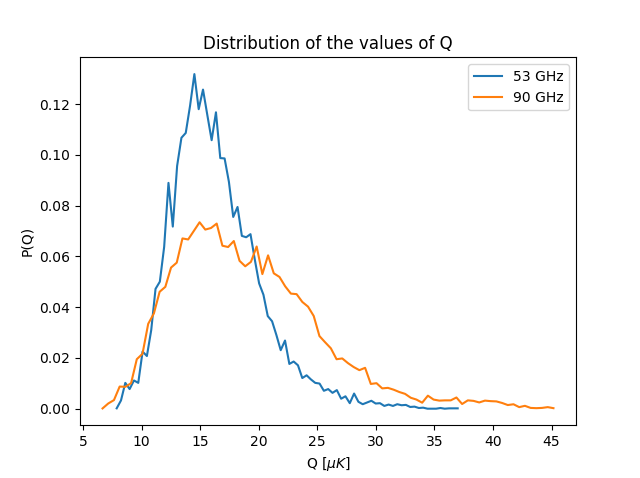
\includegraphics[scale=0.4]{mcmcJointQ.png}
}\\
\subfloat[Posterior distribution $P(n|\mathbf{d})$]{
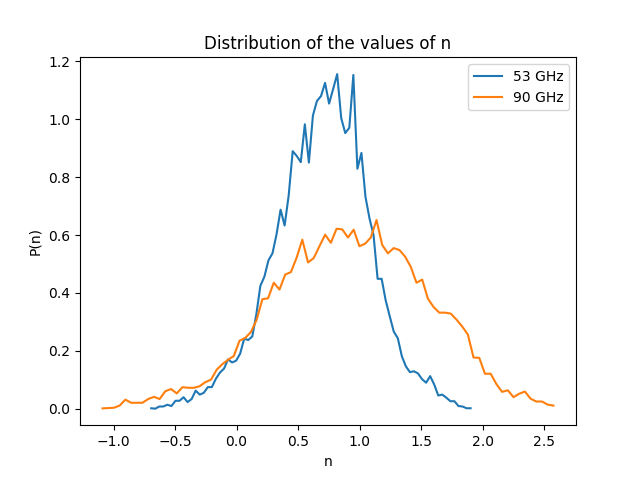
\includegraphics[scale=0.4]{mcmcJointn.png}
}
\caption{Posterior distribution $P(n|\mathbf{d})$ and $P(Q|\mathbf{d})$ with $2\cdot 10^4$ Metropolis iteration and a bin size of $250$. We have added a Savitzky-Golay filter on top of the raw data to get a clearer view of the trend.}
\label{fig:QnDist}
\end{figure}


The Monte Carlo simulations run with $2\cdot 10^4$ Metropolis iterations and take around about $80$ minutes. Due to our expectations of $Q$ and $n$, an initial guess of $Q = 20$ and $n = 1$ was made. This does not impact the results, since the Metropolis algorithm would still have found the right values if this was wrong. The result of simulation for $53$ and $90$ GHz are summarized in table \ref{tab:results}.\

The distribution plots are made with a bin size of $250$. This is done to lump close values of $Q$ and $n$ together. So the number of possible values they are allowed to have is $\#\text{Metropolis iterations}/\text{Bin Size}$. For higher bin sizes the trends are easier to see, but the fine details disappears, and for low bin sizes the details become prominent but trends are difficult to see. A bin size of $250$ seemed like the best compromise. 

The values of $Q$ and $n$ in table \ref{tab:results} are taken from the raw data, and are not affected by the bin size.









%Show the 2D likelihood contours. Summarize constraints on $Q$ and
%$n$. 


\section{Conclusions}
\label{sec:conclusions}

In this Letter we have used the $53$ and $90$ GHz maps from COBE-DMR. We have used a power-law model of the power spectrum to parametrize it with $Q$ and $n$. We then used this model and the data from COBE-DMR to calculate and optimize the posterior probability $P(Q,n|\mathbf{d})$ that the model for a given $Q$ and $n$ is correct, given the data.


$Q$ measures the fluctuation in the CMB. We hoped to find a non-zero value of $Q$, and around the theoretical $\Delta T/T \approx 10 \mu K$. The values we found was $Q = (16.3 \pm 3.81)\mu K$ for $53$ GHz and $Q = (18.9 \pm 6.12)\mu K$ for $90$ GHz. These results are more than $4\sigma$ above 0, meaning that we have statistically significant evidence that there are fluctuations in the CMB, which are in line with the predicted results of the primordial perturbations. This is strong evidence that there were differences in the early universe, which lends credence that these are the reason for the structure formation we see to day. Had the CMB been flat -- $Q \approx 0$ --, then some other mechanism had to be responsible for this.

$n$ measures the scale invariance of the fluctuations in the CMB. Inflation theory predicates a value of $n\simeq 1$. We found values of 	 This is very close to the predicted value, and this value well within the uncertainty. Since we use $\ell \leq 47$, this means that these effects should come from processes of the inflation only. Meaning that this is clear evidence for the inflation theory. 

These values were found with relatively low Metropolis iterations of $2\cdot10^4$. So multiple simulation may not give exactly the same values for $Q$ and $n$ that we found here. While this may lead to slightly different values for subsequent simulations, they should be within a standard deviation of our results. We are therefore confident that ore results are sufficiently close to the real values, that our conclusions are justified.

Given our results we have found substantial evidence for the inflationary theory of the expansion of the universe. We have evidence that there are statistical significant fluctuation in the CMB, and a near invariance of scale on these fluctuations. But: The resolutions of COBE-DMR is quite limited. So this is the most we can get from this data. Future mission are necessary to get the detailed data needed to investigate the finer structures of the CMB. Surly that will lead to a greater understanding of our universe.





%Summarize results. Discuss their importance, referring to the
%discovery to the initial seeds for structure formation. Mention that
%these results are in good agreement with expectations from
%inflationary theory.





%\begin{deluxetable}{lccc}
%%\tablewidth{0pt}
%\tablecaption{\label{tab:results}}
%\tablecomments{Summary of main results.}
%\tablecolumns{4}
%\tablehead{Column 1  & Column 2 & Column 3 & Column 4}
%\startdata
%Item 1 & Item 2 & Item 3 & Item 4
%\enddata
%\end{deluxetable}



\begin{acknowledgements}
I want to thank Aram Salihi, Hans-Petter Harveg, Andreas Helland and Markus Bjørklund for the discussion, and for the correction done text. I would also thank H. K. Eriksen and A. Drews for dealing with our relentless questioning. And a thanks also goes out to the COBE-DMR team, for that we are able to do this analysis in the first place.
\end{acknowledgements}


\bibliography{ref}



%\begin{thebibliography}{}
%
%\bibitem[G{\'o}rski et al.(1994)]{gorski:1994} G{\'o}rski, K. M.,
%  Hinshaw, G., Banday, A. J., Bennett, C. L., Wright, E. L., Kogut,
%  A., Smoot, G. F., and Lubin, P.\ 1994, ApJL, 430, 89
%
%\end{thebibliography}


\end{document}
